\section{Evaluation Suchalgorithmus}
\label{sec:suchalgorithmus}
Die Evaluation verschiedener Algorithmen zur Erkennung von Fussgängerstreifen stellte ein wichtiger Teil unserer Arbeit dar. Nach Absprachen mit unseren Dozenten und Recherchen im Internet sind wir auf die unteren Methoden zur Bilderkennung gestossen.Um die Kandidaten zu vergleichen, griffen wir auf das Werkzeug der Confusion Matrix\footnote{\url{https://de.wikipedia.org/wiki/Beurteilung_eines_Klassifikators}} (Wahrheitsmatrix) zurück.

\subsection{Algorithmen Vergleich}
Um einen neutralen Vergleich der verschiedenen Erkennungsmethoden zu erreichen, haben wir alle Methoden testweise implementiert und mit ihnen eine Erkennung im Raum Rapperswil durchgeführt.

Wir haben mit folgenden Eckdaten gearbeitet:
\begin{tabbing}[H]
    \hspace*{5cm}\=\hspace*{6cm}\= \kill
    Bounding Box (Rapperswil): \> (8.814650, 47.222553, 8.825035, 47.228935) \\
    Anzahl Fussgängerstreifen: \> 37 \\
\end{tabbing}


\subsubsection{Haar Feature-based Cascade Classifier}
\begin{figure}[H]
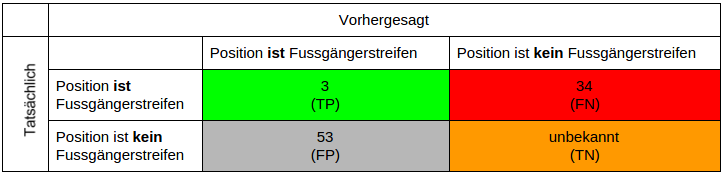
\includegraphics[width=\textwidth]{images/haar_conf.png}
\caption[Haar Feature-based Cascade Classifier]{Haar Feature-based Cascade Classifier}
\end{figure}
Auf der Suche nach möglichen Algorithmen, welche Objekte auf Bildern erkennen stiessen wir auf den Haar Feature-based Cascade Classifier. Dieser erlaubt es Objekte unabhängig von der Drehung oder Skalierung wieder zu erkennen. In einer Erweiterung von OpenCV ist der Algorithmus implementiert und kann wie in folgenden Beispiel verwendet werden: 
\begin{itemize}
	\item \url{http://coding-robin.de/2013/07/22/train-your-own-opencv-haar-classifier.html}
\end{itemize}
Für das Trainieren braucht es sehr viele Bilder und noch mehr Rechenleistung, um diese Hürden zu überwinden, schrieben wir ein Python Script, welches uns Bilder von Fussgägnerstreifen liefert. Dabei konnten wir auf OpenStreetMap Daten zurückgreifen, welche die Koordinaten von Fussgängerstreifen lieferten. Weiter stellte die HSR ihren Dev-Server zur Verfügung um die enorme Rechenleistung abzudecken. Leider wurde auch mit diversen unterschiedlichen Trainingsdaten kein brauchbares Resultat erzielt. Eine Schwierigkeit beim trainieren war, dass man kein Feedback bekam, was gute oder eher schlechtes Bildmaterial für das Training ist.

\subsubsection{Fast Fourier Transform}	
\begin{figure}[H]
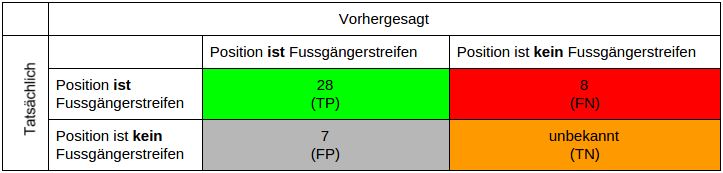
\includegraphics[width=\textwidth]{images/fast_fourier_conf.png}
\caption[Fast Fourier Transform]{Fast Fourier Transform}
\end{figure}
Die Orthofotos entlang der Strasse wurde so ausgerichtet, dass die Strasse horizontal zum Bild liegt. Der Zebrastreifen hat nun die Eigenschaft, dass wenn eine Fourier Transformation vertikal zum Bild angewendet wird, ein eindeutiges Frequenzmuster entstehen sollte. Genau genommen ist der 8. Fourierkoeffizient gegenüber seinen Nachbar erhöht (Je nach Bildqualität auch der 7. oder 9.).
Die Methode versagt jedoch, sobald der Zebrastreifen undeutlich wird, Objekte wie Autos auf dem Zebrastreifen sind oder andere Gegenstände diese dominante Frequenz auch beinhalten.
\begin{figure}[H]
	\centering
	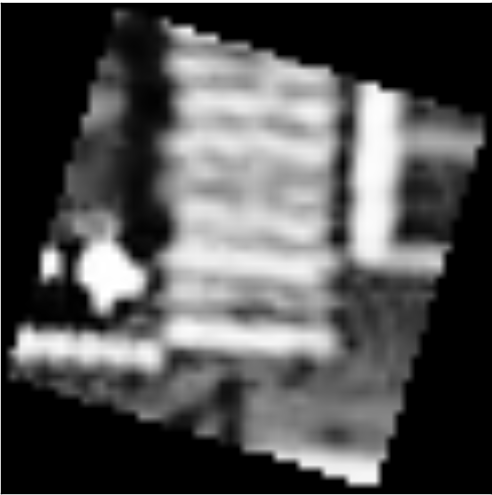
\includegraphics[width=5cm]{images/Unsharp_Crosswalk2.png}\caption[Scale-invariant Feature Transform]{Undeutlicher Zebrastreifen ohne dominanten Fourierkoeffizienten}
\end{figure}
\subsubsection{Scale-invariant Feature Transform}	
\begin{figure}[H]
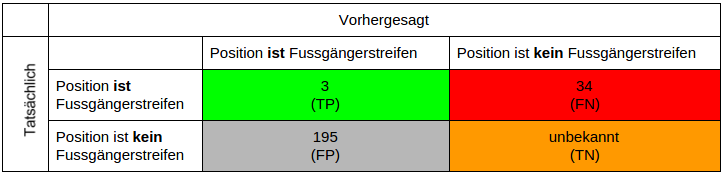
\includegraphics[width=\textwidth]{images/sif_conf.png}
\caption[Scale-invariant Feature Transform]{Scale-invariant Feature Transform}
\end{figure}
Scale-invariant Feature Transform (SIFT) ist ein Algorithmus, welcher Merkmale von Bildern beschreibt. Seine stärken sind, dass es keine Probleme mit Translation, Rotation oder Skalierung gibt. Die Idee dies Verfahrens ist jedoch mehr auf einem Bild schon bekannte Objekte wieder zu erkennen. Mit Input, welcher eine Unbekannte Situation zeigen kommt der Algorithmus nicht klar.\\
OpenCV bietet eine Implementation von SIFT, welche wir nutzten um die Evaluation durchzuführen. Das Resultat war für unsere Problemstellung alles andere als ausreichend.
\subsubsection{Deep Learning - Convnet}	
\begin{figure}[H]
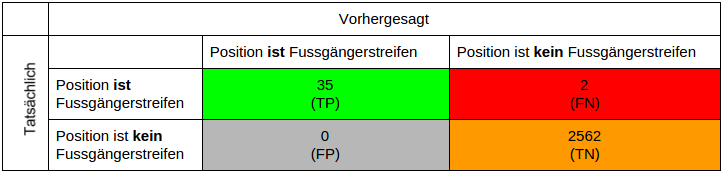
\includegraphics[width=\textwidth]{images/deep_conf.png}
\caption[Deep Learning]{Deep Learning - Convnet}
\end{figure}
Das Convolutional Neural Network (Convnet) hat die Zebrastreifen mit Abstand am besten erkannt. Anzumerken ist hier, dass die False Positive (FP) Rate von 0 ein schlichtes Zufallsergebnis ist. Wir haben diese Technik nach der Evaluation auf grösseren Flächen innerhalb der Stadt Zürich getestet und sind auf 1 FP pro 1000 Bildern gekommen. Eine Beschreibung der Technik des Covnets können sie dem nächsten Kapitel Umsetzungskonzept entnehmen.

\subsection{Auswertung}
Damit die Auswertung verständlich ist, wird hier noch auf die Berechnung und die angeführte Legende verwiesen.
\subsubsection{Legende}
\begin{tabbing}
    \hspace*{3cm}\=\hspace*{6cm}\= \kill
    TP:	\> Zahl der richtig positiven Klassifikationen\\
	FP:	\> Zahl der falsch positiven Klassifikationen\\
	TN:	\> Zahl der richtig negativen Klassifikationen\\
	FN:	\> Zahl der falsch negativen Klassifikationen\\
\end{tabbing}

\subsubsection{Berechnung}
\begin{tabbing}
    \hspace*{3cm}\=\hspace*{3cm}\=\hspace*{6cm}\= \kill
	Trefferquote \> = \> TP / (TP+FN)\\
	Richtigkeit \> = \> (TP + TN) / (TP + FP + TN + FN)\\
	Relevanz \> = \> TP / (TP + FP)\\
\end{tabbing}

\begin{table}[H]
	\centering
    \begin{tabular}{|l|l|l|l|}
    \hline    
    \rowcolor{lightblue}
	Algorithmus & Tefferquote & Richtigkeit & Relevanz \\ \hline
	Haar Feature-based Cascade Classifier & 0.08 & 0.97 & 0.05 \\ \hline
	Scale-invariant feature transform & 0.08 & 0.91 & 0.02 \\ \hline
	Fast Fourier Transform & 0.77 & 0.99 & 0.8 \\ \hline
	Deep learning & 0.95 & 0.99 & 1.0 \\ \hline
    \end{tabular}
    \caption[Algorithmen Vergleich]{Algorithmen Vergleich}
\end{table}

\decision{Evaluation Suchalgorithmus}
An dieser Stelle ist zu erwähnen, dass Bilderkennung im Allgemeinen ein nicht triviales Problem ist. Man hat mit den unterschiedlichsten Schwierigkeiten zu kämpfen, wie der Qualität oder die Belichtung der Bilder. Das führte dazu, dass nur mit dem Fast Fourier Transform und dem Deep Learning Ansatz Resultate erziehlt wurden, welche ein brauchbares Ergebnis lieferten. Der Deep Learning ist jedoch der klare Favorit und sticht insbesondere beim False Positive Wert hervor. Deshalb entschieden wir uns, unser Fokus auf diesen Algorithmus zu legen. 



